\documentclass[12pt]{article}
\setlength{\oddsidemargin}{0in}
\setlength{\evensidemargin}{0in}
\setlength{\textwidth}{6.5in}
\setlength{\parindent}{0in}
\setlength{\parskip}{\baselineskip}

\usepackage{amsmath,amsfonts,amssymb}
\usepackage[utf8]{inputenc}
\usepackage{graphicx}
\begin{document}

CS 527 Winter 2021 \hfill Homework 1\\
Hoang Vu-Kingston

\hrulefill

\begin{enumerate}
	\item\textit{Problem 1}\\
    Consider the code $\{0,01\}$
    \begin{enumerate}
        \item Is it instantaneous? Why?\\
        Not instantaneous, 01 contain 0 as prefix
        \item Is it uniquely decode-able? Why?\\
        It is uniquely decode-able, no combination of one code with itself or another can be decode as another character
        \item Is it non-singular? Why?\\
        It is non-singular, every character is encode to a different code
    \end{enumerate}
    \item\textit{Problem 2}\\
    \begin{enumerate}
        \item Binary Huffman coding\\
        \begin{align*}
            X_1 &= 1\\
            X_2 &= 00\\
            X_3 &= 011\\
            X_4 &= 01000\\
            X_5 &= 01001\\
            X_6 &= 01010\\
            X_7 &= 01011\\
        \end{align*}
        \noindent
        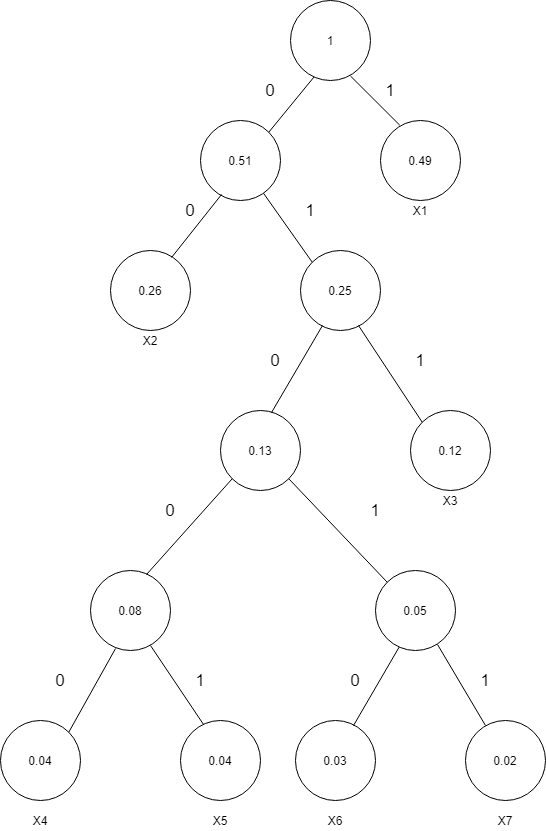
\includegraphics[width=12cm]{HW2-Q2-1.png}
        \\
        \item Expected code length\\
        \begin{align*}
            L &= |X_1|P_1 + |X_2|P_2 + |X_3|P_3 + |X_4|P_4 \\
            &+ |X_5|P_5 + |X_6|P_6 + |X_7|P_7\\
            &= 1\times0.49 + 2 \times 0.26 + 3 \times 0.12 + 5 \times 0.04\\
            &+ 5 \times 0.04 + 5 \times 0.03 + 5 \times 0.02 \\
            &= 2.02
        \end{align*}
        \item Ternary Huffman coding\\
        \begin{align*}
            X_1 &= 0\\
            X_2 &= 1\\
            X_3 &= 20\\
            X_4 &= 22\\
            X_5 &= 210\\
            X_6 &= 211\\
            X_7 &= 212\\
        \end{align*}
        \noindent
        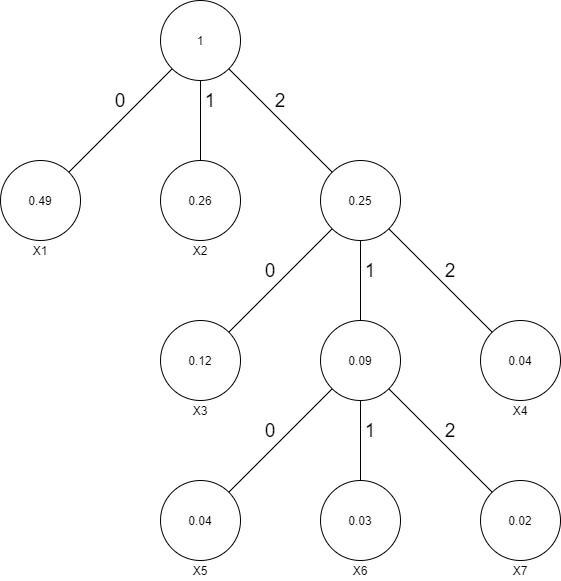
\includegraphics[width=12cm]{HW2-Q2-3.png}
        \begin{align*}
            L &= |X_1|P_1 + |X_2|P_2 + |X_3|P_3 + |X_4|P_4 \\
            &+ |X_5|P_5 + |X_6|P_6 + |X_7|P_7\\
            &= 1\times0.49 + 1 \times 0.26 + 2 \times 0.12 + 2 \times 0.04\\
            &+ 3 \times 0.04 + 3 \times 0.03 + 3 \times 0.02 \\
            &= 1.34
        \end{align*}
    \end{enumerate}
    \newpage
    \item\textit{Problem 3}\\
    $\{0,10,11\}$ is Huffman encoding for $P_X=[0.8,0.1,0.1]$\\
    $\{00,01,10,110\}$ cannot be Huffman encoding. The code 110 can be shorten to 11 without losing non-singularity. This implies there mus exist another code with prefix 11 in order for this given codes to be Huffman encoding\\
    $\{01,10\}$ is also not Huffman encoding. Similar to above, the codes can drop the last character and still preserve its non-singularity characteristic, implying that the prefix are not filled and there should be more code for it to be Huffman
    \item\textit{Problem 4}
    \begin{enumerate}
        \item Proof by contradiction\\
        For binary Huffman codes, for $p_1$ to have code length of 1, it must be that $p_1$ is the only minimum left together with the sum probability $p_2 + p_3 + p_4 + ... + p_n$.
        In contradiction, if we can find a $p_1 > 2/5$ such that it coexists with two other probabilities $p_y$ and $p_{sum}$ where $p_y$ is probability of a character Y and $p_{sum}$ is the sum of probabilities of all the other characters.\\
        Since $p_1$ is the largest probability in the list, we know that $p_y \leq p_1$\\ Furthermore, we know that in order to be encoded with length $> 1$, $p_1$ must also be one of the two minimum probability, that since the combination $p_{sum}, p_1$ can only happen if $p_y$ is greater than both, it must be the case that
        \begin{equation*}
            p_y \leq p_1 < p_{sum}
        \end{equation*}
        The 3 probabilities can be arrange as the tree show below:\\
        \\
        \noindent
        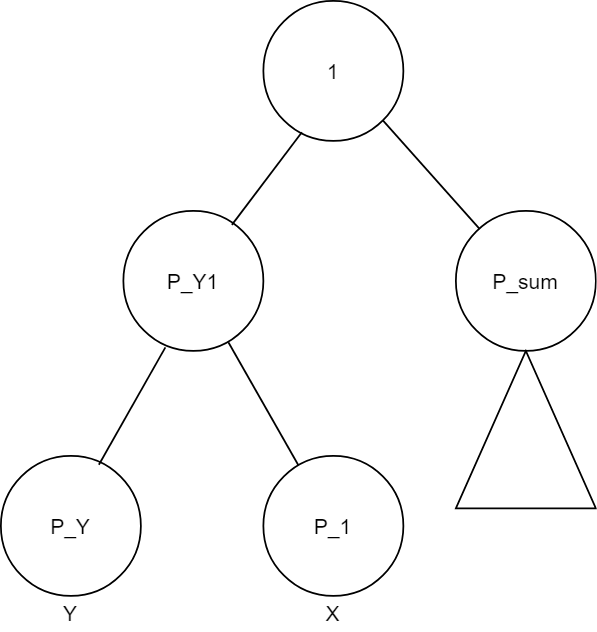
\includegraphics[width=8cm]{HW2-Q4-1.png}
        \noindent
        \\
        Where:
        \begin{align*}
            &p_1 + p_y + p_{sum} = 1 \\
            \text{and } &p_y \leq p_1 < p_{sum}\\
            \text{Since } &p_{sum} > p_1 \text{ and } p_1 > 0.4\\
            \Rightarrow &p_{sum} > 0.4\\
            \text{Since } &p_{sum} > 0.4 \text{ and } p_1 > 0.4 \text { and } p_1 + p_y + p_{sum} = 1\\
            \Rightarrow &p_y < 0.2
        \end{align*}
        Now let us split $p_{sum}$ back to its original component $[p_{sub1},p_{sub2}]$, consider the set of probabilities then of $[p_1, p_y, p_{sub1},p_{sub2}]$. Since we know $[p_{sub1},p_{sub2}]$ was selected for the next step of Huffman encoding, it must be the two lowest probabilities in the set, thus it must be lesser than $p_y$, and therefore must be lesser or equal to 0.2. However, we know that $p_{sum} > 0.4$, since $p_{sub1},p_{sub2} \leq 0.2$ this cannot happen. $p_y$ then must thus be the lowest probabilities of $< 0.2$, and thus a $p_y$ to satisfy the initial condition we assume cannot exist.\\
        By contradiction thus, $p_1$ must have length 1\\
        \item Similarly we assume again another $p_y$ exists such that the set $\{p_y,p_sum\}$ is the minimum so that $p_1$ can have length 1. The inequalities are again setup as follow:
        \begin{align*}
            &p_1 + p_y + p_{sum} = 1 \\
            &p_y,p_{sum} < p_1\\
            &p_y < p_1, p_{sum} < p_1, p_1 < \frac{1}{3}\\
            \Rightarrow &p_{sum} < \frac{1}{3}, p_y < \frac{1}{3}\\
            \Rightarrow &p_1 + p_y + p_{sum} < 1
        \end{align*}
        This again violate our assumption that the sum of these probabilities must be equal to 1, and by contradiction, the code word for $p_1$ must have length $\geq 2$
    \end{enumerate}
    \item\textit{Problem 5}
        \begin{enumerate}
            \item Best way is to drink from most likely to least likely, at the last case ($p_5$ or $p_6$) we are on our 5th drink, and can immediately deduce the bad one after that. Number of tasting required is thus:
            \begin{align*}
                N &= \frac{8}{23}1 + \frac{6}{23}2 + \frac{4}{23}3 + \frac{2}{23}4 + \frac{2}{23}5 + \frac{1}{23}5\\
                &= \frac{55}{23}
            \end{align*}
            \item The bottle with highest probability of being bad should be tasted first (aka first bottle with $\frac{8}{23}$ chance of being bad)\\
            \item Mix the two least likely probabilities every time will ensure us that the resulting average will be that of a Huffman encoding with the following tree with guarantee shortest average length of word (number of tastes):\\
            \noindent
            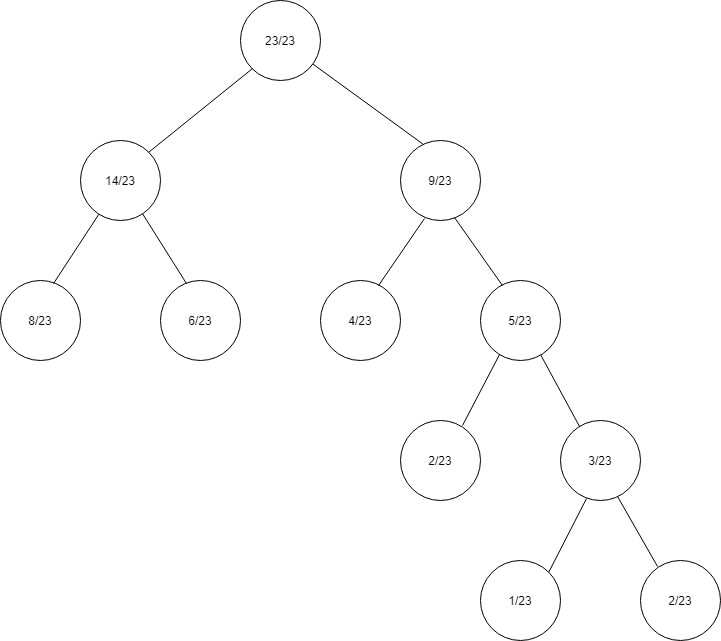
\includegraphics[width=12cm]{HW2-Q5-3.png}
            \begin{align*}
                N &= \frac{8}{23}2 + \frac{6}{23}2 + \frac{4}{23}2 + \frac{2}{23}3 + \frac{2}{23}4 + \frac{1}{23}4\\
                &= \frac{54}{23}
            \end{align*}
            To drink this, we drink the mixture according to the tree first to decided which bath to test next. For example, we drink 1 mix 2, if it bad we can drink 1 or 2 to determine which one is bad, thus bringing wine 1 and 2 to 2 drink to test. If it good, we can immediately deduce the other batch of 3456 is bad, according to the tree, 3456 is 456 mix with 3, we drink 3 after knowing 1 mix 2 is good to determine whether 3 is bad or 456 is bad. So on and so forth
    \end{enumerate}
    \newpage
    \item\textit{Problem 6}
    \begin{enumerate}
        \item Floating point conversion to decimal use \textit{BaseForm} function provided by \textit{Mathematica}\\
        \begin{center}
            \begin{tabular}{ c  c  c  c  c }
                 &  $P_i$ & $F_i$ & $l_i$ & code \\
                 & 0.5 & 0 & 1 & 0\\
                 & 0.25 & 0.5 & 2 & 10\\
                 & 0.125 & 0.75 & 3 & 110\\
                 & 0.125 & 0.875 & 3 & 111\\
            \end{tabular}
        \end{center}
        \item We know that\\
        \begin{align*}
            H(X) &= \sum_{i=1}^{n} p_ilog(\frac{1}{p_i})\\
            &= \sum_{i=1}^{n} p_il_i
        \end{align*}
        Note that the average length of this code is also\\
        \begin{equation*}
            L = \sum_{i=1}^{n} p_il_i\\
        \end{equation*}
        But since the average length require each code word to have integer length, $l_i$ is always round up to the nearest integer $\lceil l_i \rceil \geq l_i$, and thus
        \begin{equation}
            H(X) \leq L
        \end{equation}
        Observe also that
        \begin{align*}
            \lceil log(\frac{1}{p_i}) \rceil &< log(\frac{1}{p_i}) \\
            \Rightarrow \lceil l_i \rceil &< l_i +1\\
            \Rightarrow \sum_{i=1}^{n} p_i\lceil l_i \rceil &< \sum_{i=1}^{n} p_i(l_i + 1)\\
            \Rightarrow L &< \sum_{i=1}^{n} p_il_i + \sum_{i=1}^{n} p_i\\
            \Rightarrow L &< \sum_{i=1}^{n} p_il_i + 1
        \end{align*}
        And thus:
        \begin{equation}
            L < H(X) + 1
        \end{equation}
        by (1) and (2):
        \begin{equation*}
            H(X) \leq L < H(X) + 1
        \end{equation*}
        Prefix proof:\\
        Consider the nature of Shannon coding basing itself on negative power of 2, and consider the code for two character $X_i$ and $X_j$ (where $i < j$) with probabilities $[p_i,p_j]$, pre-binary conversion, the code for them are:
        \begin{align*}
            F_i &= \sum_{k=1}^{i-1} p_i\\
            F_j &= \sum_{k=1}^{j-1} p_j
        \end{align*}
        Because the nature of prefix code, $F_j$, the longer code cannot contain $F_i$. In other words, the first $l_i$ characters of $F_j$ must be different from $F_i$, we can write this as the inequality:
        \begin{align*}
            &F_j - F_i > 2^{-l_i}\\
            LHF&=  F_j - F_i\\
            &=p_i + p_{i+1} + ... + p_{j-1} + p_j \\
            RHS&= 2^{-l_i}\\
            &=2^{-log_2(\frac{1}{p_i})}\\
            &=2^{log_2(p_i)}\\
            \Rightarrow & F_j - F_i > 2^{-l_i} \text{ is always true}
        \end{align*}
        Thus, the Shannon coding is prefix code
    \end{enumerate}
\end{enumerate}

\end{document}
